\chapter{Badania eksperymentalne i uzyskane wyniki}
Przeprowadzenie skanowania domen z dostarczonego zbioru danych zajęło 11 dni, co poskutkowało zebraniem około 30GB informacji na
temat analizowanych serwerów. Przeskanowano cały plik wejściowy liczący około 5 miliardów pozycji. Skanowanie przeprowadzone było
w dniach od 21. kwietnia 2017 roku do 1. maja 2017 roku włącznie.

Obciążenie skanera zwiększano stopniowo w ciągu kolejnych dni przeprowadzania skanowania. W ten sposób można było uniknąć przeciążenia
skanera oraz uzyskać jednocześnie zadowalającą wydajność. Okazało sie, że możliwe jest uruchomienie większej liczby procesów niż
przewidywano na etapie projektowania. Przełożyło się to na krótszy czas skanowania.

\section{Typy odebranych odpowiedzi}\label{sec:typy}
Wśród przeanalizowanych par domen i serwerów można zaobserwować kilka charakterystycznych typów odpowiedzi. Odpowiedzi mogą być
dzielone na kategorie ze względu na różne kryteria. Pierwszym kryterium, które będzie brane pod uwagę w niniejszej pracy jest
rozmiar pliku przechowującego informacje pobrane z serwera autorytatywnego. Jest to motywowane faktem, że w istocie im większy
jest plik z odpowiedzią, tym spodziewamy się, że zawiera on więcej informacji na temat odpytywanej domeny.

Pierwszym typem jest odpowiedź, która zajmowała na dysku specyficzną ilość miejsca -- 25123 bajty. Zaobserwowano, że uzyskano
626288 odpowiedzi tego typu. Rozmiar pliku jest swego rodzaju skutkiem ubocznym uproszczonej implementacji skanera. Trudno było
przewidzieć wszystkie specyficzne przypadki towarzyszące transferowi strefy DNS. Zaobserwowana sytuacja jest właśnie jednym z
tych nietypowych sytuacji i nawet program dig nie odwzorowuje idealnie zachowania jakie powinno nastąpić w takiej sytuacji.
Przyczyną utworzenia opisanego wcześniej pliku nie jest jednoznacznie określona. Zostały podjęte próby ustalenia czym spowodowane
	jest takie zachowanie. W takich samych przypadkach program dig zwraca jedynie rekord DNS SOA i komunikat o błędzie (ang.
\textit{communications error: end of file}). Zachowanie programu dig w dużym stopniu przypomina przekierowanie zapytania IXFR na
AXFR (ang. \textit{AXFR fallback}) opisane między innymi w RFC1995 \cite{RFC1995}. Wywołanie mechanizmu AXFR fallback następuje
w sytuacji, kiedy numer wersji pliku strefy przysłany do serwera jest wyższy niż numer wersji aktualnie na nim przechowywany.
Na różnego rodzaju forach \cite{powerdns-forum} czy w serwisach internetowych \cite{powerdns-git}, problem który został opisany
pojawia się najczęściej jako problem implementacji oprogramowania PowerDNS \cite{powerdns}. Niemniej jednak nie ustalono dokładnie
jaki jest powód wysłania pakietu powodującego takie zachowanie w odpowiedzi na zwykłe zapytanie AXFR.

Kolejnym przykładem odpowiedzi, która powodowała powstanie dużego pliku na dysku, było odebranie od serwera autorytatywnego pakietu
TCP RST(ang. \textit{TCP reset packet}). Sytuacja taka wynika również z pewnego uproszczenia, które zostało przyjęte w implementacji
skanera. Założono, że zawsze zostanie odebrany pakiet DNS. Podyktowane było to ograniczonym czasem w którym implementowano skaner
oraz faktem, że problem ten można w łatwy sposób obejść poprzez odfiltrowanie odpowiednich plików w katalogu z wynikami. Dodatkowo
sytuacje tego typu były bardzo sporadyczne, więc nie wpływało to w znaczącym stopniu ani na czas przeanalizowania pobranych danych
ani na wynik tej analizy.

Kolejnymi specyficznymi grupami jeśli chodzi o rozmiar pliku z odpowiedzią są już typowe odpowiedzi na zapytania AXFR.
Najmniejszy rozmiar mają oczywiście odpowiedzi, które zawierają jedynie rekord SOA i jest to dopuszczalna odpowiedź na zapytanie
AXFR. Następnie, wraz ze zwiększającą się liczbą wpisów w pliku strefy DNS, zwiększa się rozmiar odpowiedzi. Nie przekłada się to
jednak bezpośrednio na informacje, które można wyodrębnić z takich plików strefy. Zdarza się bowiem sytuacja, w której znaczną część
pliku strefy DNS zajmują wpisy podpisów cyfrowych RRSIG, których długość przekłada się na rozmiar plików. Dodatkowo, podpisy
generowane mogą być dla każdego rekordu oddzielnie (co szerzej opisano w podpunkcie \ref{TSIG}), dlatego też wpływa to bardzo
znacząco na rozmiar otrzymywanej odpowiedzi.

\section{Odebrane adresy IPv4 oraz IPv6}
\label{sec:adresy_ip}
Częstym argumentem, który pojawia się podczas dyskusji na temat bezpieczeństwa transferów plików bazy danych DNS jest ujawnianie
adresów IP. W niniejszym podrozdziale skupiono się głównie na adresach IP w wersji 4. ponieważ jest to wciąż dominujący typ adresacji
w Internecie \cite{Ipv6_deployment}. Okazuje się, że pomimo obaw o wycieki adresów przez dokonywanie nieuprawnionego transferu nikt nie
zbadał dokładnie jak duża może być skala tego zjawiska. Umożliwiły to badania przeprowadzone w tej pracy magisterskiej.

Aby nie ograniczać się tylko do jednego typu adresacji urządzeń, zostały oddzielone i przeanalizowane dwa zbiory danych -- dla IPv4
oraz dla IPv6. Głównym celem analizy adresów IP było ustalenie systemów autonomicznych(ang. \textit{AS -- Autonomous System}),
z których pochodzą określone maszyny. Następnie możliwe było, na podstawie numerów AS, określenie kraju w którym dane maszyny są
zlokalizowane.

\subsection{Analiza AS}
Podstawową informacją, którą uzyskać można wykorzystując pobrane dane z transferów AXFR, jest przynależność otrzymanych adresów IP
do konkretnych grup autonomicznych. Grupy te określają przynależność do sieci, które zarządzane są przed tego samego operatora
sieciowego, a wykorzystuje się je głównie w protokołach routingu. Informacje związane z systemami autonomicznymi można, w głównej
mierze, znaleźć w RFC1930 \cite{RFC1930}. Zbiór danych został podzielony ze względu na wersję protokołu IP używanej przy adresacji
konkretnych maszyn. Przeprowadzono analizę systemów autonomicznych w rozdzielnych grupach, dla wersji 4 protokołu IP oraz dla wersji 6.

Jak już wcześniej wspomiano (rozdział \ref{sec:adresy_ip}), wciąż dominującym sposobem adresacji urządzeń w sieci jest adresacja
IP w wersji 4 \cite{Ipv6_deployment}.
Do podobnych wniosków można dojść analizując zbiór dannych zebranych podczas skanowania. Okazuje się bowiem, że znaczna większość
adresów IP, które zostały pobrane w wyniku skanowania należy do zbioru adresów IP w wersji 4. Dane liczbowe prezentują się w
następujący sposób:
\begin{enumerate}
	\item znaleziono 1695653 adresów publicznych adresów IPv4 -- oznacza to, że odflitrowano te adresy, które zostały określone
	jako adresy sieci prywatnych w RFC1918 \cite{RFC1918},
	\item odflitrowano 127424 adresów IPv6, które są różne od adresu ,,localhost'' (:::::::1) -- zgodnie z wymaganiami postawionymi
	w RFC4291 \cite{RFC4291}.
\end{enumerate}

\subsection{Sposób określenia AS}
W celu określenia numerów systemów autonomicznych adresów IP pozyskanych podczas skanowania zaimplementowane zostalo kolejne
narzędzie umożliwiające takie mapowanie. Społeczność udostępnia kilka sposobów dopasowania adresów IP do odpowiadających im
systemów autonomicznych. Podczas badań zapoznano się z dwoma z nich, które opisano poniżej:
\begin{enumerate}
	\item API udostępnione przez Team Cymru \cite{cymru},
	\item biblioteka języka Python pyasn \cite{pyasn}.
\end{enumerate}

Pierwszy ze sposobów jest prostszy w użyciu, gdyż wystarczy użyć narzędzia netcat \cite{netcat}, gdzie argumentami jest odpowiednia
strona internetowa Team Cymru \cite{cymru} oraz ścieżka do pliku, w którym znajdują się w kolejnych liniach adresy IP. Każdy z plików
rozpoczyna się słowem kluczowym ,,begin'' oraz kończy słowem kluczowym ,,end''. Sposób ten jest wygodny, jednak moze budzić pewne
wątpliwości. Najbardziej istotną wydaje się być kwestia dotycząca głównie adresacji IP w wersji 4. -- dynamiczne przydzielanie adresów
IP różnym operatorom \cite{RFC2050}. Problem związany jest pośrednio z kończącą sie pulą adresów IPv4. Prowadzi to do zmian przynależności
adresów IPv4 do systemów autonomicznych. Dynamikę tych zmian można obserwować między innymi pod adresem \cite{cidr_report}.

Wątpliwości, które wynikły z wykorzystania udostępnionego API były bezpośrednią przyczyną szukania innego, optymalnego rozwiązania.
Takim okazało się wykorzystanie biblioteki \textit{pyasn} \cite{pyasn}. Umożliwia ona zaimplementowanie narzędzia, które uwzględnia
datę, gdy dany adres IP został zeskanowany. Mapowanie adresu IP na AS w konkretnym dniu jest możliwe dzięki wykorzystaniu wielu baz
danych. Okazuje się, że w praktyce, dla każdej z dat udostępniony jest oddzielny plik z bazą danych, dzięki której możliwe jest
tłumaczenie adresów IP na ASy. Możliwe jest pobranie bazy danych, która najlepiej odpowiada zebranym pomiarom. W przypadku niniejszej
pracy magisterskiej pobierane są pliki dla każdego dnia, w którym przeprowadzone zostało skanowanie. Pliki są dystrybuowane wraz z
biblioteką. Użytkownik musi przygotować pliku tekstowego z datami, dla których powinna zostać
pobrana baza danych. Następnie bazy są przetwarzane na pliki w formacie odpowiednim dla biblioteki \textit{pyasn}. Aby zautomatyzować
opisany proces, zaimplementowano odpowiednie narzędzie w języku skryptowym bash, którego działanie zaprezentowano na diagramie
\ref{fig:netcat}. Pobiera ono daty z odpowiednich katalogów z wynikami
skanów, następnie tworzy odpowiedni plik tekstowy, który później wykorzystywany jest jako plik wejściowy dla biblioteki \textit{pyasn}.
Na jego podstawie kopiowane są bazy danych dla konkretnych dni. Pobrane bazy danych są następnie konwertowane do takiego formatu,
którego wymaga narzędzie. W kolejnym kroku dokonuje się właściwego odwzorowania adresów IP na odpowiadające im ASy.
\begin{figure}[h]
	\centering
	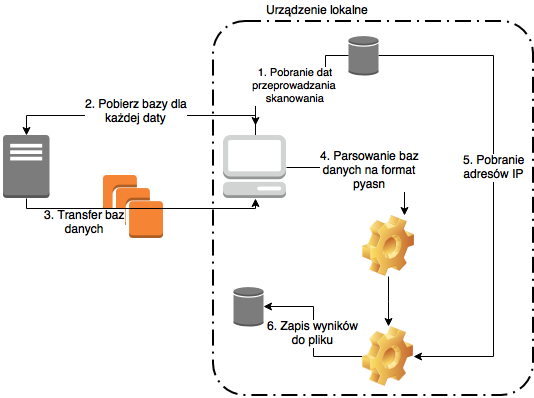
\includegraphics[width=1.0\textwidth]{image/netcat}
	\caption{Zasada działania narzędzia mapującego adresy IP na numery AS.}
	\label{fig:netcat}
\end{figure}

Jest to bardziej dokładna forma mapowania adresów IP na numery
systemów autonomicznych. Translacja uzależniona jest od bazy danych, której wersję określa użytkownik. API, które zostało opisane
na początku tego rozdziału jest całym komponentem, na który użytkownik nie ma wpływu. Dodatkowo, w przypadku poprzedniego systemu,
do interfejsu serwera nie jest przekazywana data, więc należy zakładać, że adresy IP są mapowane na numery systemów autonomicznych
na podstawie najnowszej bazy danych. Aby odwzorowanie było jak najbardziej wiarygodne, mapowanie adresów powinno być realizowane
już w dniu przeprowadzania skanowania, co dodatkowo obciążyłoby serwer i przełożyło się na niższą wydajność.

\subsection{Zbiór adresów IPv4}
\label{sec:ipv4_results}
Analizując zbiór pod kątem adresów IP jedynie w czwartej wersji, zaprezentowany na rysunku \ref{fig:ipv4_countries}, możemy
zauważyć kilka interesująych faktów. Pierwszym, który jest natychmiast zauważalny, to bardzo wysoki współczynnik systemów autonomicznych
ze Stanów Zjednoczonych w populacji adresów IPv4 które zostały zebrane w wyniku skanowania. Poziom ten jest około 3.5 raza wyższy,
niż liczebność systemu autonomicznego z drugiego kraju w rankingu, czyli z Niemiec. Informacja ta jest interesująca w tym sensie, że
TLD .de jest jedną z tych, które wymagają zabezpieczania stref DNS przed \textit{zone enumeration} \cite{euLaw, zoneEnumeration}.
Okazuje się natomiast,
że w praktyce drugim najczęściej spotykanym krajem w zestawieniu adresów IP w skanowaniu AXFR są właśnie Niemcy, a transfer strefy
jest w realizacji dużo łatwiejszym atakiem niż wspomniane wcześniej \textit{zone walking} \ref{zone_enumeration}.

Dodatkowo, zastanawiające jest, że oprócz bardzo widocznej przewagi systemów autonomicznych ze Stanów Zjednoczonych, widoczna jest
również duża różnica pomiędzy 9 pierwszymi krajami oraz resztą populacji (etykieta \textit{tr} (Turcja) na
wykresie \ref{fig:ipv4_countries}).

\begin{figure}[h]
	\centering
	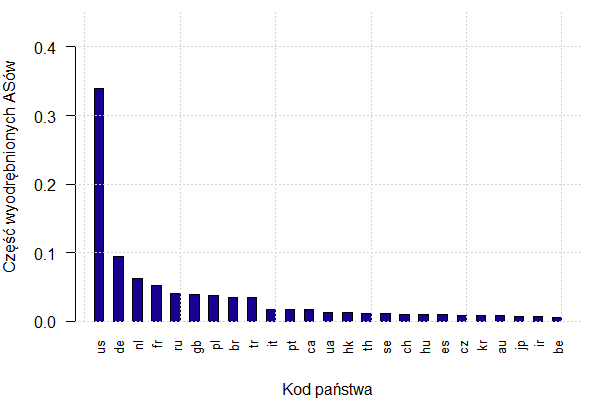
\includegraphics[width=1.0\textwidth]{image/ipv4_as_countries_no_title}
	\caption{Pochodzenie geograficzne adresów IPv4 z podziałem na państwa. Adresy określane na podstawie numerów AS.}
	\label{fig:ipv4_countries}
\end{figure}

\begin{figure}[h]
	\centering
	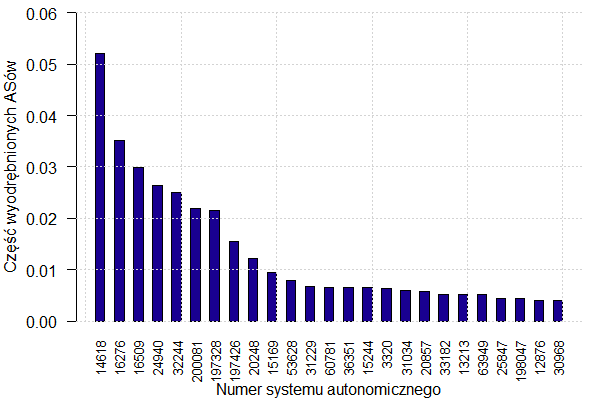
\includegraphics[width=1.0\textwidth]{image/asn_all_no_title}
	\caption{Zestawienie systemów autonomicznych, z których domeny najczęściej odpowiadają na zapytania AXFR.}
	\label{fig:asn_all}
\end{figure}

\subsection{Zbiór adresów IPv6}
Oprócz opisanego w poprzednim podpunkcie \ref{sec:ipv4_results} przeanalizowano zebrane dane pod względem zawartości adresów IP
w wersji 6. Rozpatrując przypadek adresów IPv6 widzimy na rysunku \ref{fig:ipv6_as_countries} wyraźną przewagę systemów autonomicznych
z trzech państw -- Niemiec, Turcji oraz Holandii. Z pewnością wpływ na zaprezentowane wyniki miał również stopień zaawansowania
wdrożenia IPv6 w poszczególnych państwach. Zastanawiająca jest stosunkowo niska pozycja systemów autonomicznych ze Stanów Zjednoczonych,
jednak można przypuszczać, że jest to właśnie konsekwencja stanu wdrożenia protokołu IPv6. Kolejne z państw przestawione na
wykresie \ref{fig:ipv6_as_countries} stanowią już bardzo małą część wszystkich systemów autonomicznych -- nawet poniżej 1\textperthousand.
\begin{figure}[h]
	\centering
	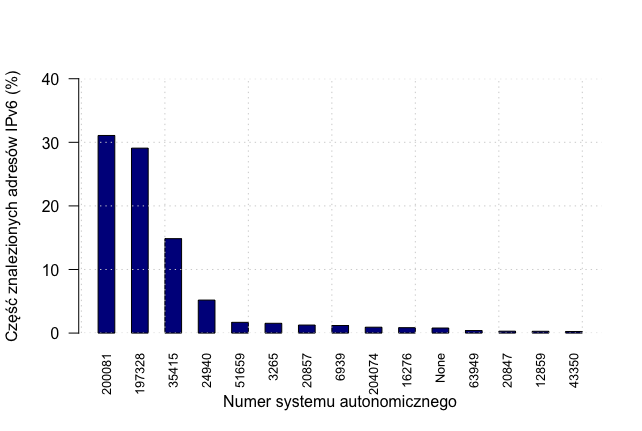
\includegraphics[width=1.0\textwidth]{image/ipv6_countries_no_title}
	\caption{Pochodzenie geograficzne adresów IPv6 z podziałem na państwa. Adresy określane na podstawie numerów AS.}
	\label{fig:ipv6_as_countries}
\end{figure}

Analogicznie jak w przypadku opisanym w rozdziale \ref{sec:ipv4_results} zaprezentowano bardziej szczegółowy wykres, na podstawie
którego możliwa jest analiza adresów ze wzlęgu na numery poszczególnych systemów autonomicznych. Widać dość wyraźną różnicę pomiędzy
dwoma najbardziej licznymi zbiorami AS, a całą resztą znalezionych adresów. Co więcej, są to systemy autonomiczne stosunkowo młode,
na co wskazują ich wysokie indeksy (20081 i 197328).
\begin{figure}[h]
	\centering
	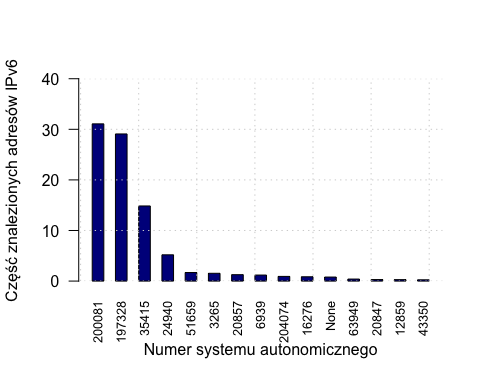
\includegraphics[width=1.0\textwidth]{image/Ipv6_as_count_no_title}
	\caption{Pochodzenie geograficzne adresów IPv6 z podziałem na państwa. Adresy określane na podstawie numerów AS.}
	\label{fig:ipv6_co}
\end{figure}

\section{Analiza TLD}
Jednym z podejść analizy zebranego zbioru danych było sprawdzenie, jak przedstawia się rozkład popularności domeny najwyższego poziomu
dla serwerów podatnych na nieuprawiony transfer strefy.

W głównej mierze należy zastanowić się, czy rozkład ten jest w ogóle istotny, czy może nie różni się on niczym od ogólnego,
całościowego rozkładu popularności TLD w internecie, bez uwzględnienia podatności, czy innych czynników. W tym celu przeanalizowano
i przedstawiono wykres popularności domen najwyższego poziomu w sieci Internet \cite{TLD_popularity}. Jest on przedstawiony na
rysunku \ref{fig:TLD_all}.
\begin{center}
	\begin{figure}
		\centering
		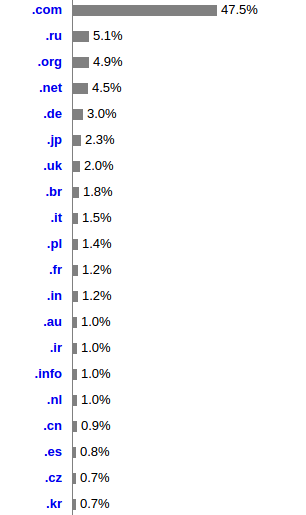
\includegraphics[scale=0.75]{image/TLD_all}
		\caption{Popularność TLD w internecie (dostęp na dzień 15. maja 2017), źródło:  \cite{TLD_popularity}.}
		\label{fig:TLD_all}
	\end{figure}
\end{center}

Wykres przedstawia procentowy rozkład poszczególnych domen internetowych w zależności od używanej domeny najwyższego poziomu.
Wynika z niego, że domena najwyższego poziomu \textit{.com} jest używana przez 47.5\% wszystkich domen. Wykres ograniczony został
do 20 najbardziej popularnych TLD. Różnice pomiędzy kolejnymi rekordami są na tyle niskie, że ich umieszczenie wpływałoby negatywnie
na ogólną reprezentację wyników. Wykres \ref{fig:TLD_all} zostanie następnie zestawiony z popularnością TLD tych domen, których serwery
autorytatywne umożliwiają nieuprawniony transfer AXFR. Rozkład popularności TLD domen odpowiadających na zapytanie AXFR przedstawiono
na rysunku \ref{fig:resp}.
\begin{center}
	\begin{figure}
		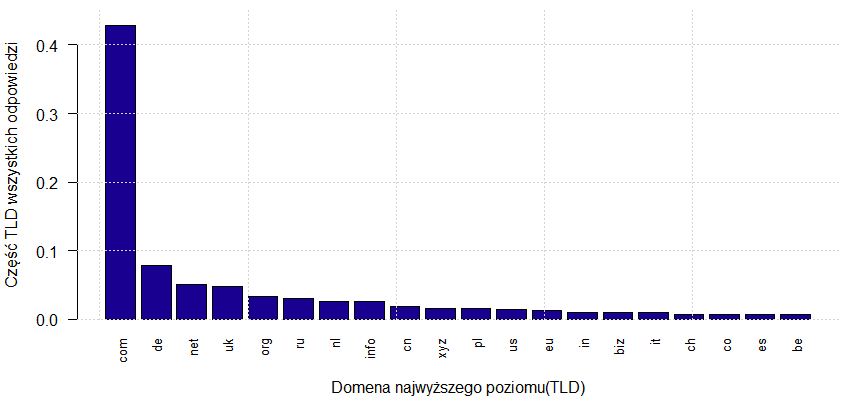
\includegraphics[width=1.0\textwidth]{image/resp_no_title}
		\caption{Popularność TLD w odpowiedziach AXFR.}
		\label{fig:resp}
	\end{figure}
\end{center}

Dokonując porównania wykresów \ref{fig:TLD_all} oraz \ref{fig:resp} możemy dostrzec kilka prawidłowości. Zarówno w jednym jak i
drugim przypadku, wyraźnie dominującą domeną najwyższego poziomu jest domena .com. Dodatkowo, nie można mówić tu o anomalii,
ponieważ zarówno w jednym jak i drugim przypadku domena .com stanowi bardzo podobny procentowy udział wszystkich domen, czy to
pytanych czy tych, które odpowiedziały. Następnie można dostrzec delikatne zmiany w procentowych udziałach kolejnych TLD, jednak
nie na pierwszy rzut oka zmiany te nie są wyróżniające się czy nad wyraz zauważalne.

W związku z tym, że wyżej opisane działania nie pozwoliły na wyraźne zarysowanie różnic pomiędzy rozkładami TLD, zdecydowano się
zestawić ze sobą inne zbiory danych. Wykreślono podobne wykresy dla popularności domeny najwyższego poziomu dla domen odpytywanych
podczas skanowania oraz TLD domen, które na zapytania odpowiedziały. Następnie zestawiono ze sobą wyniki pozyskane z obu tych zbiorów
danych. Zostały odpowiednio wykreślone:
\begin{enumerate}
	\item wykres 15 najpopularniejszych TLD w zbiorze domen odpytywanych w porównaniu do popularności tych TLD w zbiorze domen,
	które odpowiedziały na zapytanie AXFR -- wykres \ref{req_to_resp},
	\item wykres 15 najpopularniejszych TLD w zbiorze domen, które odpowiedziały na zapytanie AXFR w zestawieniu z ich popularnością
	w puli TLD domen odpytywanych -- wykres \ref{resp_to_req}.
\end{enumerate}

\begin{figure}[h]
	\centering
	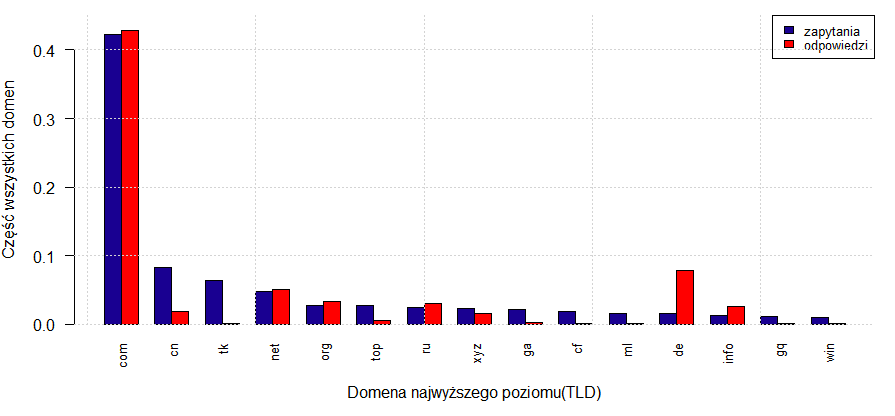
\includegraphics[width=1.0\textwidth]{image/req_to_resp_no_title}
	\caption{Zestawienie odpowiedzi ze względu na rozkład danych wejściowych. Rozkład odpowiedzi znormalizowano do całkowitej liczby
	odpowiedzi, zaś rozkład zapytań do całkowitej ich liczby.}
	\label{req_to_resp}
\end{figure}

\begin{figure}[h]
	\centering
	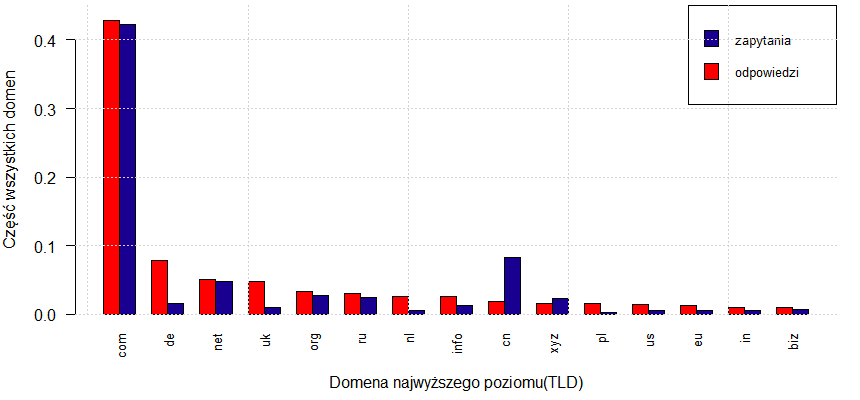
\includegraphics[width=1.0\textwidth]{image/resp_to_req_no_title}
	\caption{Zestawienie częstości występowania domen najwyższego poziomu dla domen, dla których możliwy jest AXFR z ich populacją
	w zbiorze danych wejściowych. Rozkład odpowiedzi znormalizowano do całkowitej liczby
	odpowiedzi, zaś rozkład zapytań do całkowitej ich liczby.}
	\label{resp_to_req}
\end{figure}

W przypadku tych bezpośrednich zestawień, można zauważyć więcej interesujących prawidłowości. Na początku warto wspomnieć, że
istnieje duża dysproporcja w przypadku niektórych domen najwyższego poziomu. Pierwszą z nich może być przypadek domeny .de,
gdzie procentowy udział TLD .de we wszystkich TLD odpowiedzi AXFR jest drugim wynikiem podczas, gdy w populacji danych wejściowych
jest to 12 najliczniejsza grupa. Warto dodać, że domena .de jest jedną z domen, których zarządcy traktują proceder
\textit{zone enumeration} jako łamanie prawa, co opisano w podpunkcie \ref{zone_enumeration}. Transfer AXFR pozwala na uzyskanie
danych o podobnej charakterystyce, a mimo to, ok 8\% wszystkich odpowiedzi powiązane jest z domeną najwyższego poziomu .de
(domena krajowa -- Niemcy). Podobna sytuacja ma miejsce również w przypadku TLD .uk (Wielka Brytania) czy .pl (Polska),
gdzie przy małym współczynniku domen odpytywanych otrzymano nieproporcjonalnie wysoki współczynnik odpowiedzi.

Zjawiskiem w pewnym stopniu odwrotnym do opisanego w poprzednim akapicie jest rozkład zapytań/odpowiedzi dla TLD .cn (Chiny)
lub .tk (Tokelau -- region zależny od Nowej Zelandii). W tym przypadku zauważalna jest również duża dysproporcja, jednak
,,na korzyść'', gdyż w stosunku do wielu zapytań wystosowanych do domen należących do tych TLD uzyskano relatywnie mało odpowiedzi.
Domena .tk jest interesującym przykładem również z innego względu. Jej operator -- DotTK umożliwia rejestrację darmowych domen.
W związku z taką polityką, TLD .tk stała się bardzo popularna wśród cyberprzestępców. W 2007 roku firma McAfee uznała ją za najbardziej
niebezpieczną spośród wszystkich domen \cite{mcafee2007}. W 2010 roku domena ta znalazła się znacznie niżej w rankingu \cite{mcafee2010}, jednak wciąż
była to wysoka, jedenasta pozycja. W obu raportach domena .cn również znajduje się na wysokich miejscach.
Również TLD .top można zaliczyć do domeny o niskiej proporcji zapytań względem odpowiedzi. Została ona oficjalnie wydzielona
w 2014 roku. Jej operatorem jest firma ,,.top registry'' znajdująca się w Chinach, a domeny zarejestrowane w TLD .top muszą używać
chińskich serwerów.

Oprócz opisanych wcześniej względnych porównań pomiędzy pytaniami i odpowiedziami od serwerów autorytatywnych różnych domen
sprawdzono jak wygląda dystrybuanta poszczególnych rozkładów. Pozwoliło to oszacować ile (ilościowo) domen najwyższego poziomu
zawierało się w grupie, dla której generowano większość zapytań (rysunek \ref{cdf_tld_req}). Analogicznie, w przypadku danych
dotyczących odpowiedzi AXFR można było ocenić ile różnych TLD pojawia się niemal we wszystkich odpowiedziach (rysunek \ref{cdf_tld_resp}).

\begin{figure}[h]
	\centering
	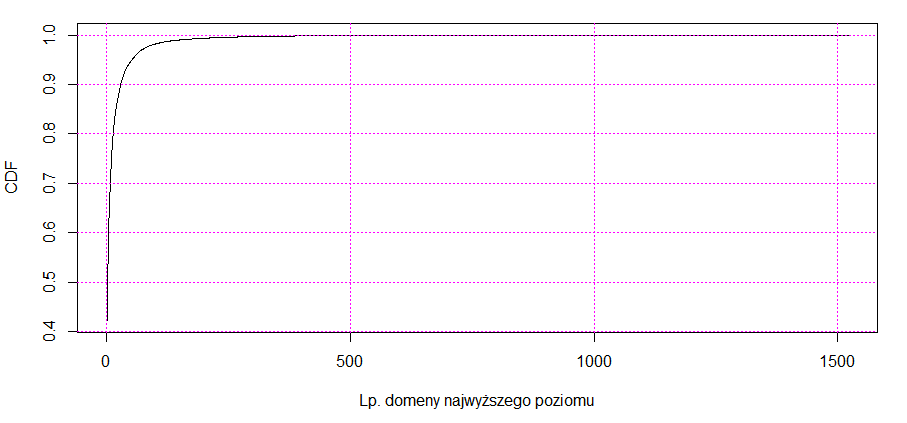
\includegraphics[width=1.0\textwidth]{image/cdf_tld_req_no_title}
	\caption{Dystrybuanta domeny najwyższego poziomu w odpytywanych domenach.}
	\label{cdf_tld_req}
\end{figure}

\begin{figure}[h]
	\centering
	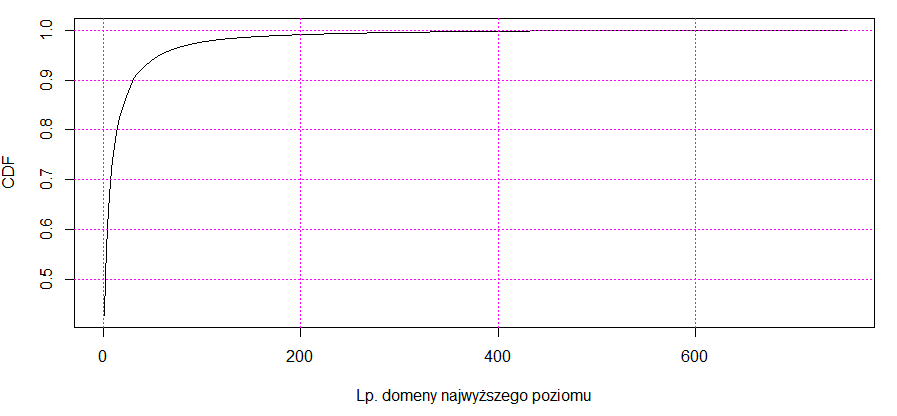
\includegraphics[width=1.0\textwidth]{image/cdf_tld_resp_no_title}
	\caption{Dystrybuanta domeny najwyższego poziomu w zbiorze domen odpowiadających strefą DNS na zapytanie AXFR.}
	\label{cdf_tld_resp}
\end{figure}


Oprócz wykreślonych charakterystyk policzono również ile domen najwyższego poziomu gromadzi w sobie 99\% zapytań bądź odpowiedzi
(w zależności od badanego zbioru). Wyniki zaprezentowano w tabeli \ref{cdf_table}. Warto zauważyć, że pomimo ponad dwukrotnie
mniejszego zbioru różnych domen poziomu najwyższego, należy zgrupować dużo więcej TLD, aby uzyskać zbiór 99\% wszystkich odpowiedzi.
Można z tego wnioskować, że rozkład odpowiedzi jest bardziej jednostajny niż w przypadku danych wejściowych. Można także przypuszczać,
że zbiór wejściowy zawierał pojedyncze domeny z różnych, rzadko spotykanych TLD. W momencie, kiedy jedna, czy jedynie kilka domen
z takiego TLD są odpowiednio zabezpieczone przed nieuprawnionym transferem AXFR nie znajdziemy danego sufiksu w zbiorze odpowiedzi.
Sytuacja taka może mieć miejsce, gdy wszystkie domeny z mało popularnego TLD znajdują się pod zarządem jednej osoby czy organizacji.

\begin{table}[h]
	\centering
	\caption{Opis zbiorów zapytań/odpowiedzi}
	\label{cdf_table}
	\begin{tabular}{|p{0.2\textwidth}|p{0.3\textwidth}|p{0.4\textwidth}|}
		\hline
		\textbf{Zbiór} &
		\textbf{Liczba różnych TLD w zbiorze} &
		\textbf{Liczba różnych TLD zawierająca 99\% elementów zbioru} \\
		\hline\hline
		Zapytania &
		1521 &
		147\\
		\hline
		Odpowiedzi &
		751 &
		187\\
		\hline
	\end{tabular}
\end{table}

\section{Liczba wpisów stref w odpowiedziach}
Odpowiedzi pobrane w wyniku skanowania zostały poddane analizie uwzględniającej jak duże są strefy pobrane z serwerów przestrzeni nazw.

W tym przypadku zastosowano inne podejście niż podczas reszty przeprowadzonych badań. Z racji tego, że częstym przypadkiem odpowiedzi
otrzymywanej od serwera był jedynie rekord SOA/CNAME, postanowiono oddzielnie analizować pliki stref zawierające tylko jeden wpis, a
oddzielnie pliki zawierające więcej niż jeden rekord.

W wyniku przeprowadzonych badań ustalono, że:
\begin{enumerate}
	\item 6179845 z 8985154 (68,8\%) plików stref zawiera jedynie jeden wpis (rekord SOA bądź rekord CNAME),
	\item 2803902 z 8985154 (31,2\%) plików stref zawiera więcej niż jeden wpis.
\end{enumerate}
Przypadek, gdy plik strefy zawiera więcej niż jeden wpis można utożsamić ze źle skonfigurowanym serwerem autorytatywnym domeny.
Zwracanie samego wpisu SOA (czyli odpowiednik zbioru danych z jednym wpisem w pliku strefy) nie może być traktowane jako błąd,
gdyż w dokładnie taki sam sposób zachowuje się serwer DNS w przypadku podania błędnego numeru serii w transferze IXFR. Tak
zaprojektowany został inkrementalny transfer strefy DNS zaprezentowany w RFC1995 \cite{RFC1995} i do tej pory nie zaprezentowano
ewentualnych podatności, które mogłyby wykorzystywać ten protokół.

Dla zbioru danych, który określa rozmiar pobranych stref wykreślony został histogram, z którego można odczytać, jak często spotykane
są strefy DNS o określonych rozmiarach. W przypadku skanów polegających na transferze stref widoczna jest bardzo duża częstość
występowania domen o wpisach do kilkudziesięciu rekordów. Pierwszy z histogramów na których zaprezentowano opisane częstości
(rysunek \ref{fig:hist_zone_size}) sugeruje, że dużo bardziej interesująca jest pierwsza część całego wykresu. Zaprezentowano ją,
w powiększeniu, na kolejnym rysunku \ref{fig:hist_zone_size_zoom}. Dodatkowo, w górnej części rysunku \ref{fig:hist_zone_size}
umieszczono histogram w powiększeniu, z bardzo ograniczoną skalą na osi rzędnych. Pozwala to, na zaobserwowanie prążków, które
nie były widoczne na histogramie prezentującym cały zbiór.

\begin{figure}[h]
	\centering
	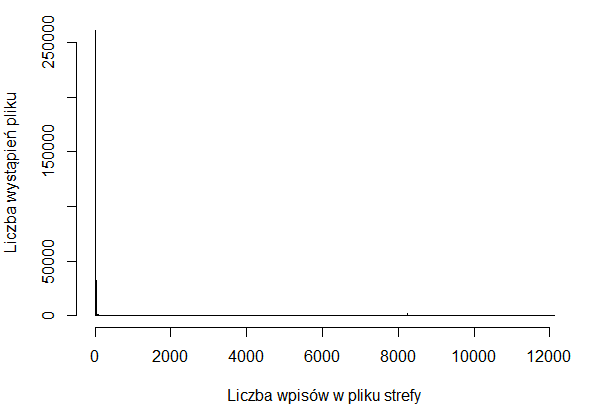
\includegraphics[width=1.0\textwidth]{image/hist_zone_size_no_title}
	\caption{Rozkład liczby rekordów w odpowiedziach AXFR.}
	\label{fig:hist_zone_size}
\end{figure}

\begin{figure}[h]
\centering
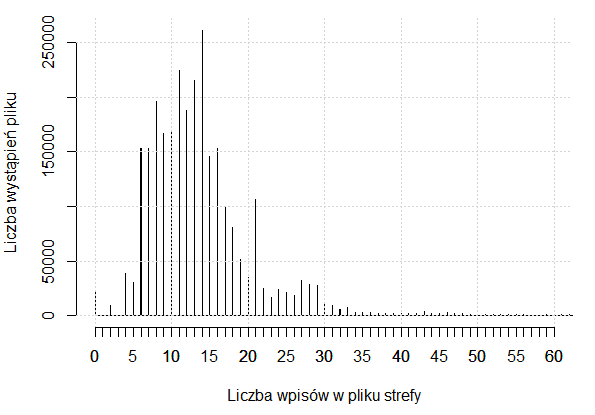
\includegraphics[width=1.0\textwidth]{image/hist_zone_size_zoom_no_title}
\caption{Rozkład liczby rekordów w odpowiedziach AXFR, widok powiększony.}
\label{fig:hist_zone_size_zoom}
\end{figure}

Dodatkowo, można zauważyć, że histogram \ref{fig:hist_zone_size} posiada bardzo dużo pozycji na osi X. Jest to ponownie następstwo
własnej implementacji oprogramowania umożliwiającego transfer stref AXFR. Zauważalny jest prążek na wartości około 8 tysięcy
wpisów. Dokładnie jest to 8244 wpisów w pliku strefy. Sprawdzono, czy rzeczywiście strefy te są tak duże. Odpytano kilka z serwerów,
dla których otrzymano tak specyficzną odpowiedź. Pakiety, które wysłano oraz odebrano zostały przeanalizowane programem Wireshark.
Okazuje się, że utworzenie opisanego wcześniej pliku jest następstwem otrzymania wiadomości HTTP o statusie 400 -- Bad request.
Co ciekawe, odpowiedź tę otrzymujemy na mało standardowy port w kontekście protokołu HTTP -- port 53. Szczegóły otrzymanej wiadomości
zostały przedstawione w lsitingu \ref{list:dnsHTTPstd}. Innym wynikiem typu zachowania były odpowiedzi o liczbie linii ok. 11 tysięcy.
Jest to wyraźnie mniej zauważalne, wnioskując choćby po histogramie \ref{fig:hist_zone_size}, gdzie widoczny jest jedynie prążek na
wartości około 8000 linijek w pliku strefy. Plik o około 11 tysiącach (11900 linii) wpisów był tworzony w wyniku otrzymania rozszerzonej,
głównie o tagi HTML wiadomości HTTP 400 -- została ona przedstawiona na listingu \ref{list:dnsHTTPmore}.

\begin{lstlisting}[label={list:dnsHTTPstd},captionpos=b,caption=Odpowiedź HTTP 400 na zapytanie DNS.,language=xml]
HTTP/1.0 400 Bad request
Cache-Control: no-cache
Connection: close
Content-Type: text/html

<html><body><h1>400 Bad request</h1>
Your browser sent an invalid request.
</body></html>
\end{lstlisting}

\begin{lstlisting}[label={list:dnsHTTPmore},captionpos=b,caption=Rozszerzona odpowiedź HTTP 400 na zapytanie DNS.,language=xml]
<html>
<head><title>400 Bad Request</title></head>
<body bgcolor="white" >
<center><h1>400 Bad Request</h1></center>
<hr><center>nginx/1.4.0</center>
</body>
</html>
\end{lstlisting}

Na rysunku \ref{fig:hist_zone_size_zoom} możemy obserwować w przybliżeniu rozkład wielkości plików stref. Zawężony został on do 60
wpisów z uwagi, że najbardziej interesujące wyniki zawierają się głównie w tym przedziale. Jak widać, najczęściej występującym
rozmiarem strefy DNS jest 14 wpisów. Są to strefy pobrane najczęściej ze źle skonfigurowanych serwerów DNS, które obsługują usługi
standardowe, często spotykane, takie jak serwery WWW, serwer pocztowe. Przykład odpowiedzi o takim rozmiarze został przedstawiony na
listingu \ref{list:dns_zone_example}.

\begin{lstlisting}[label={list:dns_zone_example},captionpos=b,caption=Przykładowa odpowiedź na żądanie strefy DNS.,language=bash]
movida-bar.pl.  14400   6        ns1.consultingteam.pl. hostmaster.movida-bar.pl. 1952801133 3222735464 1869837421 1634956389 1925188727
movida-bar.pl.  14400   15      mail.movida-bar.pl
movida-bar.pl.  14400   16      v=spf1 a mx ip4:91.241.61.119 ~all
movida-bar.pl.  14400   1       91.241.61.119
movida-bar.pl.  14400   2       ns1.consultingteam.pl
movida-bar.pl.  14400   2       ns2.consultingteam.pl
ftp.movida-bar.pl.      14400   1       91.241.61.119
localhost.movida-bar.pl.        14400   28      0000:0000:0000:0000:0000:0000:0000:0001
localhost.movida-bar.pl.        14400   1       127.0.0.1
mail.movida-bar.pl.     14400   1       91.241.61.119
pop.movida-bar.pl.      14400   1       91.241.61.119
smtp.movida-bar.pl.     14400   1       91.241.61.119
www.movida-bar.pl.      14400   1       91.241.61.119
movida-bar.pl.  14400   6        ns1.consultingteam.pl. hostmaster.movida-bar.pl. 2013010900 14400 3600 1209600 86400
\end{lstlisting}

Z listingu \ref{list:dns_zone_example} możemy dowiedzieć się, że domena obsługiwana przez odpytany serwer DNS udostępnia między
innymi takie usługi jak serwery pocztowe smtp i pop, serwer FTP oraz serwer WWW. Wszystkie one są kierowane na jeden adres IP.
Dodatkowo, na serwerze DNS został umieszczony wpis TXT (id 16). Zdefiniowano w nim rekord SPF gdzie określa się reguły dotyczące
wymiany wiadomości e-mail w danej domenie. Odwzorowanie indeksów poszczególnych rekordów DNS można odczytać z tabelii \ref{records}.

Strefy tego typu są najczęściej spotykane w danych, które udało się zebrać podczas skanowania. Można wnioskować, że transfer AXFR
jest najczęściej możliwy dla domen zarejestrowanych głównie w celach informacyjnych czy marketingowych. Jak opisano wcześniej, są
to najczęściej pojedyncze adresy IP z kilkoma usługami. Działalność organizacji, na potrzeby których rejestowano takie niewielkie
domeny, jest najczęściej mało związana z informatyką czy telekomunikacją.

To, na co warto zwrócić uwagę na histogramie \ref{fig:hist_zone_size_zoom} to również domeny o strefach o rozmiarze około 40-60 wpisów.
Jest to reprezentacja tych stref, które wykorzystują mechanizm podpisywania rekordów DNS zaprezentowany w rozszerzedniu
protokołu -- DNSSEC \cite{RFC4034, RFC4035}. Zgodnie z tym, co zostało opisane w rozdziale \ref{tsig}. Dla każdej pary rekordów
przechowywanych w strefie DNS liczony jest podpis cyfrowy. Serwery, które odpowiedziały strefą zawierającą podpisy kryptograficzne
najprawdopodobniej wspierają DNSSEC, co może zostać użyte przez cyberprzestępców do

\section{Odpowiedzi niestandardowe}
Jak wspomniano w podpunkcie \ref{sec:typy}, wyjątkową sytuacją, którą udało się zaobserwować, były odpowiedzi o nietypowym
rozmiarze 25123 bajtów. Przykładowa komunikacja z serwerem odpowiadającym w ten sposób została zaprezentowana na listingu
\ref{list:unused}.

\begin{lstlisting}[label={list:unused},captionpos=b,caption=Przykładowy odpowiedź serwera.,language=bash]
mskwarek\$ dig tnttelivision.com @173.255.218.70 axfr

; <<>> DiG 9.8.3-P1 <<>> tnttelivision.com @173.255.218.70 axfr
;; global options: +cmd
tnttelivision.com.	86400	IN	SOA	ns1.parklogic.com. hostmaster.tnttelivision.com. 2017061500 16384 2048 1048576 2560
;; communications error to 173.255.218.70#53: end of file
\end{lstlisting}

W tym samym czasie ustawiono nasłuchiwanie programu Wireshark \cite{wireshark} na odpowiednim interfejsie oraz odfiltrowano ruch sieciowy
nie związany z komunikacją z serwerem przestrzeni nazw o adresie 173.255.218.70. Ogólny przebieg komunikacji można zobaczyć na
zrzucie ekranu \ref{fig:unused_wireshark}.
\begin{figure}[h!]
\centering
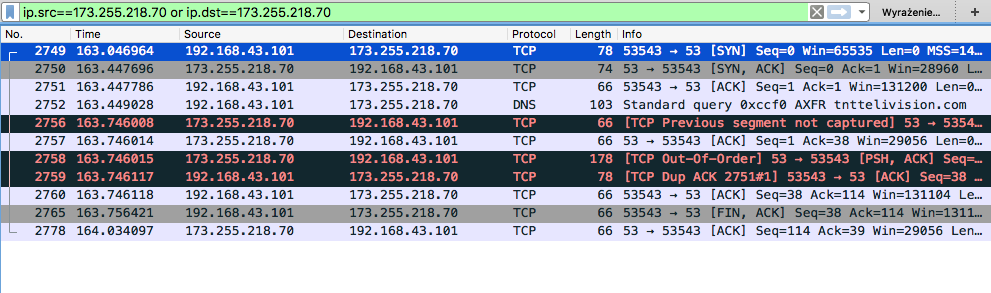
\includegraphics[width=1.0\textwidth]{image/unused_wireshark}
	\caption{}
\label{fig:unused_wireshark}
\end{figure}

Postanowiono sprawdzić, czy domeny oraz serwery autorytatywne powiązane z takimi przypadkami mają
wspólne cechy. Pierszym kryterium porównania wspomnianych przypadków była analiza systemów autonomicznych, do których przynależą
dane serwery przestrzeni nazwy. Wyniki zaprezentowano w tabeli \ref{tab:unused}.
\begin{table}[h]
	\centering
	\caption{Tabela liczebności AS w opisywanym przypadku}
	\label{tab:unused}
	\begin{tabular}{|p{0.2\textwidth}|p{0.5\textwidth}|p{0.2\textwidth}|}
		\hline
		\textbf{Numer AS} &
		\textbf{Nazwa AS} &
		\textbf{Liczba wystąpień} \\
		\hline\hline
		63949 & LINODE-APLinode, LLC, US & 324483 \\
		\hline
		32181 & ASN-GIGENET-GigeNET, US & 168263 \\
		\hline
		2516 & KDDI KDDI CORPORATION, JP & 133523 \\
		\hline
		4837 &  CN & 290 \\
		\hline
		29676 & GRADWELL, GB & 8 \\
		\hline
		263632 & BR & 6 \\
		\hline
		46844 & ST-BGP-Sharktech, US & 2 \\
		\hline
		44682 & TELECOMROMANIA Strada Peroninr.45, RO & 2 \\
		\hline
		12876 & AS12876, FR & 2 \\
		\hline
		701 & UUNET-MCI Communications Services, Inc. d/b/a VerizonBusiness, US & 1 \\
		\hline
		45413 & SERVENET-AS-TH-AP Serve NET Solution Limited Partnership, TH & 1 \\
		\hline
		12374 & LFNET-AS01, DE & 1 \\
		\hline
	\end{tabular}
\end{table}

Niewątpliwie interesującym zjawiskiem jest fakt, że znaczna większość tych specyficznych plików pochodzi z kilku ASów.
Może to sugerować, że właśnie w tych systemach autonomicznych operatorzy wykorzystują oprogramowanie specjalnie modyfikowane
pod swoje potrzeby, jednak nie zawsze zgodne ze specyfikacją ustalaną w kolejnych dokumentach RFC. Wynik zapytania, który zaprezentowano
na listingu \ref{list:unused} zawiera rekord SOA, który wskazuje, że podstawowym serwerem dla tej domeny jest
serwer \textit{ns1.parklogic.com}. Nazwa tego serwera może sugerować, że dana domena została zaparkowana. \cite{todo:koniecznie}

Na wykresie \ref{fig:unused_pie} pokazano procentowy rozkład krajów z których pochodziły serwery przestrzeni nazw. Jak widać,
serwery z jedynie dwóch krajów (Japonii oraz Stanów Zjednoczonych) stanowią liczną grupę w tym zestawieniu. Pozostałe kraje, nawet
zebrane we wspólną grupę stanowią zaledwie 0,5\textperthousand.

\begin{figure}[h]
\centering
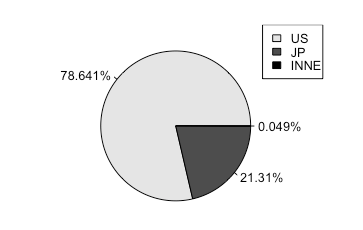
\includegraphics[width=1.0\textwidth]{image/unused_pie_no_title}
\caption{Lokalizacja serwerów nazw odpowiadających pakietem TCP z flagą RST.}
\label{fig:unused_pie}
\end{figure}

Przedstawiona proporcja jest ciekawa w kontekście analizy domen najwyższego poziomu, które obsługują serwery nazw opisane
w poprzednim akapicie. Jeśli chodzi o ten zbiór, to różnorodność jest zdecydowanie większa. Wciąż najbardziej popularną domeną
jest .com, kojarzona w głównej mierze ze Stanami Zjednoczonymi. .....

\section{Geograficzna lokalizacja serwerów}
Biorąc pod uwagę poprzednie rozważania postanowiono, że warto przeanalizować geograficzne rozmieszczenie serwerów przestrzeni nazw,
które odpowiedziały na zapytanie AXFR. Podział zaprezentowany w tym punkcie jest już bardziej szczegółowym rozbiciem konkrentych
wyników. Najważniejszym kryterium podziału domen było przede wszystkim rozdzielenie plików stref oraz odpowiadających im serwerów
przestrzeni nazw w zależności od tego jak duży plik strefy udało się dla nich pozyskać.

Pierwszym wykresem który zaprezentowano jest mapa adresów IP serwerów przestrzeni nazw, które odpowiedziały plikiem strefy zawierającym
więcej niż jeden rekord DNS. Należy dodać, że pliki ,,sztuczne'', takie, które powstały w wyniku niedoskonałości napisanego oprogramowania
nie zostały uwzględnione podczas niniejszej analizy. Wyniki zaprezentowano na rysunku \ref{fig:many_lines_map}.

\begin{figure}[h]
\centering
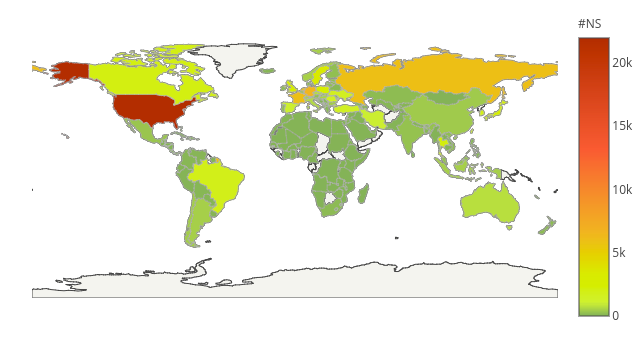
\includegraphics[width=1.0\textwidth]{image/many_lines_map_no_title}
\caption{Lokalizacja serwerów DNS, które odpowiedziały więcej niż jednym rekordem.}
\label{fig:many_lines_map}
\end{figure}

Zbiór adresów IP serwerów przestrzeni nazw który zaprezentowano na mapie \ref{fig:many_lines_map} liczył 109160 unikalnych adresów, podczas
gdy zbiór wszystkich plików stref danego typu dla analizowanego zbioru wynosił 2132448. Oznacza to, że na jeden serwer autorytatywny
średnio przypada ponad 19 domen. Wykreślona została dystrybuanta rozkładu popularności serwerów przestrzeni nazw odpowiadających na
zapytania AXFR. Przedstawiono ją na rysunku \ref{fig:cdf_ns}. Widoczna jest na nim ciekawa tendencja, że odpowiedzi o połowie
wszystkich domen, dla których pobrano informacje, pochodzą od relatywnie niewielkiej liczby serwerów przestrzeni nazw. Dokładne
kwantyle przedstawionego rozkładu zawarto w tabeli \ref{tab_cdf_ns}.

\begin{figure}[h]
\centering
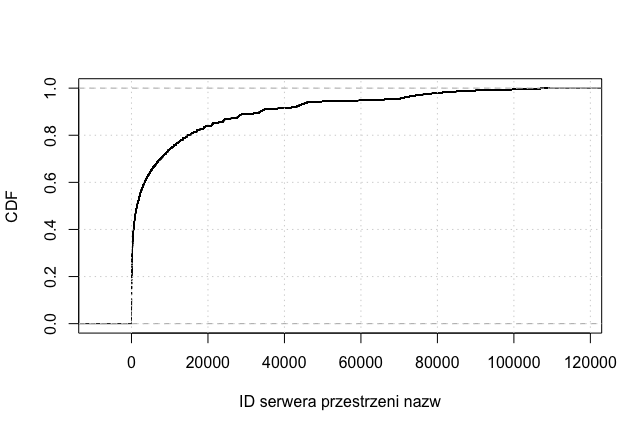
\includegraphics[width=1.0\textwidth]{image/cdf_ns_responded}
\caption{Dystrybuanta rozkładu popularności serwerów przestrzeni nazw, które odpowiadają na zapytania AXFR.}
\label{fig:cdf_ns}
\end{figure}

Z danych zawartych w tabeli \ref{tab_cdf_ns} wynika, że 75\% (trzeci kwantyl) wszystkich domen, które umożliwiają transfer strefy
obsługiwanych jest przez jedynie 9.69\% autorytatywnych serwerów przestrzeni nazw. Trend ten jest również zauważalny na wykresie
dystrybuanty \ref{fig:cdf_ns}, gdzie od poziomu 0,75 na osi OY charakterystyka jest bardziej łagodna niż w pozostałej części wykresu.
Wyniki te oznaczają, że dla pozostałych 25\% domen autorytatywnych jest 90,21\% wszystkich serwerów przestrzeni nazw. Najpopularniejsze
adresy IP serwerów NS zapisano również w tabeli \ref{tab:most_cnt_ns} wraz z liczbą domen, dla których dany serwer jest autorytatywnym.


\begin{longtable}{|c|p{3cm}|p{3cm}|}
	\hline
	\textbf{Kwantyl} &
	\textbf{Liczba serwerów} &
	\textbf{Procent wszystkich serwerów} \\
	\hline\hline
	I & 136 & 0,12\% \\
	II & 1447 & 1,33\% \\
	III & 10579 & 9,69\% \\
	IV & 109160 & 100\% \\
	\hline
	\caption{Kwantyle rozkładu popularności serwerów przestrzeni nazw, które odpowiadają na AXFR.}
	\label{tab_cdf_ns}
\end{longtable}
\begin{longtable}{|c|p{3cm}|p{3cm}|}
	\hline
	\textbf{Lp.} &
	\textbf{Adres IP} &
	\textbf{Liczba domen} \\
	\hline\hline
	1 & 167.160.13.69 & 16503 \\
	2 & 167.160.13.70 & 16318 \\
	3 & 162.243.45.236 & 14254 \\
	4 & 199.255.159.226 & 13735 \\
	5 & 198.204.224.146 & 13439 \\
	6 & 173.208.189.26 & 13222 \\
	7 & 209.160.33.82 & 13153 \\
	8 & 104.219.19.52 & 13113 \\
	9 & 192.151.149.92 & 12602 \\
	10 & 101.200.203.5 & 10659 \\
	\hline
	\caption{Autrytatywne NS dla największej liczby domen.}
	\label{tab:most_cnt_ns}
\end{longtable}

\section{Usługi}
Przeprowadzone skanowanie umożliwiło również sprawdzenie jakie usługi uruchamiane są wewnątrz organizacji, których serwery DNS
były odpytywane. Zdecydowano się na sprawdzanie usług typowych dla branży ICT. Poszukiwano w zebranych danych informacji o serwerach
systemów kontroli wersji (git, svn) oraz systemów automatycznego budowania oprogramowania i zapewniania ciągłej integracji (jenkins).
W niniejszej pracy magisterskiej zdecydowano się głównie na te usługi ze względu na dużą wrażliwość takich danych jak kody źródłowe
przechowywane na serwerach git czy svn a także ze względu na istotę elementów środowiska pracy jak systemy CI typu Jenkins.

Dodatkowo sprawdzono jak często w odebranych strefach możliwe jest znalezienie informacji na temat usług pocztowych. W tym przypadku
głównym celem poszukiwań były wpisy typu MX (id: 15) definiujące serwery wymiany poczty elektronicznej w danej domenie. Oprócz
wcześniej wspomnianych usług, postanowiono także sprawdzić popularność serwerów wymiany plików ftp.

\subsection{Usługi wspomagające rozwój oprogramowania}
Jeśli chodzi o usługi, które zostały wymienione w pierwszym akapicie tego rozdziału, to na podstawie samego adresu URL udało się
uzyskać informacje o ponad 3 tysiącach serwerach systemu git oraz ponad 3.5 tysiącach systemów svn. W odniesieniu do skali
przeprowadzonych badań jest to nieduża liczba, co dobrze świadczy o społeczności. Niemniej jednak, liczba około 7 tysięcy systemów
kontroli wersji, o których informacje uzyskano jedynie poprzez skanowanie AXFR jest wysoką liczbą. Szczególnie, jeśli uwzględniony
zostanie fakt, że systemy te najczęściej wykorzystywane są przez osoby o wykształceniu technicznym, które są świadome istoty
bezpieczeństwa sieciowego.

Kolejną z wymienionych usług był serwer CI Jenkins. Jest to jeden z najpopoularniejszych systemów ciągłej integracji. Filtrując
wyniki po adresach URL zdobyto informacje o 1.5 tysiąca serwerów tego typu.

\subsection{Usługi poczty elektronicznej}
Z zeskanowanych danych można również pozyskiwać informacje o usługach poczty elektronicznej. Wyróżniono kilka podejść do
poszukiwania takich informacji. Jednym z nich jest poszukiwanie adresów domen z prefiksem \textit{owa}.
Odpowiadają one najczęściej systemom pocztowym firmy Microsoft (ang. \textit{Outlook Web Access}) i często, dla ułatwienia
zapamiętania adresu tej usługi, skraca się jej adres do właśnie tego skrótu. Innym podejściem jest pobieranie ze stref DNS rekordów
o identyfikatorze równym 15, czyli serwerów wymiany poczty.

W niniejszej pracy magisterskiej zdecydowano się na przeprowadzenie analizy zarówno jedną jak i drugą opisaną metodą. Wyniki zostały
zaprezentowane poniżej:
\begin{itemize}
		\item znaleziono 3378 rekordów, które odnoszą się do serwisów \textit{Outlook Web Access}; są to rekordy typu A, AAAA lub
		CNAME, więc odnoszą się odpowiednio do adresów IPv4, adresów IPv6 lub są zwykłymi aliasami dla innych domen,
		\item zostały wyodrębnione 3443626 rekordów typu MX (id 15); oprócz typowego zastosowania rekordu MX, czyli definiowania
		serwerów poczty elektronicznej wewnątrz domeny zauważono, że niektóre ze znalezionych wpisów odnoszą się do usług pocztowych
		firmy Google.
\end{itemize}

Specyficzny rekord MX, który odnosi się do usług firmy Google jest najczęściej postaci \textit{alt\{id\}.aspmx.l.google.com} lub
\textit{aspmx\{id\}.googlemail.com}. Obecność takiego wpisu w strefie DNS sugeruje, że ogranizacja, która wykorzystuje daną domenę
korzysta z usług określanych nazwą \textit{G Suite}. Nazwa odnosi się głównie do usług poczty elektronicznej dla firm udostępnianych
przez Google jak również do rozwiązań Cloud -- edycji czy przechowywania dokumentów w chmurze.

Oprócz tego, że informacje na temat usług poczty elektronicznej są istotne ze względów czysto infrastrukturalnych, czyli cyberprzestępca
pozyskuje informacje na temat uruchomionego serwera poczty, to mogą być również ciekawe ze względu na możliwość użycia ich w atakach
phishingowych. Niewątpliwie informacja taka jak typ używanego systemu pocztowego (\textit{Outlook Web Access}, \textit{G Suite} czy
inne) są istotną informacją dla takiego ataku i pozwalają lepiej się do niego przygotować.


\section{Wpisy SPF}
Wpisy SPF zostały zdefiniowane w celu ochrony użytkowników domeny przed spamem. Pozwalają na określanie reguł, czy wiadomość
elektroniczna powinna zostać przyjęta przez serwer czy nie.

Istotnym elementem wpisów SPF są między innymi kwalifikatory. Wyróżniamy kwalifikatory: ,,+'', ,,-'', ,,?'', ,,~''. Szczególnie
interesujący jest kwalifikator +all, który mówi, że reguły SPF pozwalają na odebranie wszystkich wiadomości ze wszystkich domen.
Wśród danych pobranych podczas skanowania znaleziono 1.8 miliona wpisów SPF. Co ciekawsze, 3.5 tysiąca z nich było opatrzonych
klauzulą ,,+all''. Daje to między innymi bardzo ciekawą informację dla osób wysyłających niechcianą pocztę (tzw. spam). Wiedząc,
że reguły SPF nie odfiltrują danej wiadomości warto jest próbować wysyłać ją do użytkowników mających adres w danych domenach.

\section{Strefy ISP}
Podczas realizacji pracy magisterskiej zauważono w zebranych danych obecność specyficznych domen, których rozmiar wynosił od
250 do 260 wpisów.
